\subsection{Point estimate}
\label{sec:etas-point}

In a perfect world, it would be possible to predict precisely when a bus will arrive at a stop and display this single number to passengers. Alas, as we have seen, arrival time prediction is prone to significant levels of uncertainty. However, since much of the infrastructure currently only allows for point estimates, we present some here. We now examine if it is possible to find a single statistic that performs well---on average---and, more importantly, is more reliable than the currently deployed schedule-delay method.




\begin{knitrout}\small
\definecolor{shadecolor}{rgb}{0.969, 0.969, 0.969}\color{fgcolor}\begin{figure}

{\centering 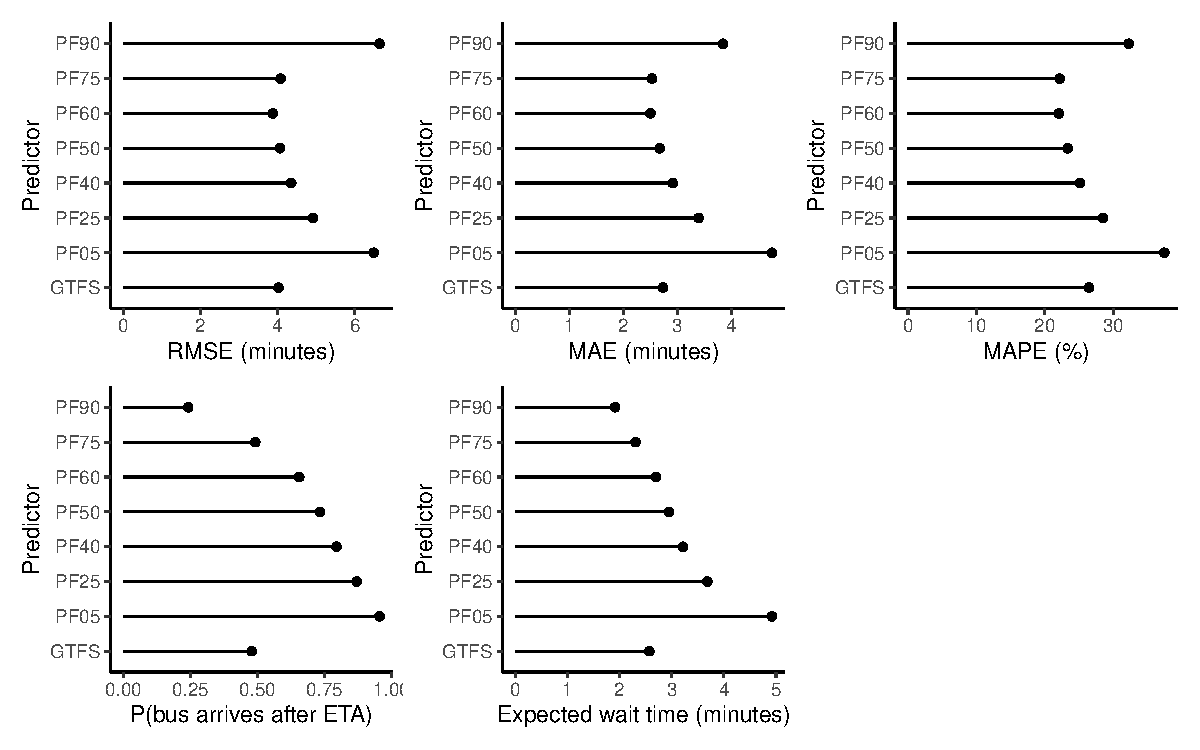
\includegraphics[width=.7\textwidth]{figure/eta_overall_results-1} 

}

\caption[Comparison of the summary statistics for various quantiles of the predictive distribution and the scheudle-delay method]{Comparison of the summary statistics for various quantiles of the predictive distribution (PFX uses the X\% quantile) and the currently deployed schedule-delay (SD) method. Results are obtained using off-peak data (between 9h30 and 14h30).}\label{fig:eta_overall_results}
\end{figure}


\end{knitrout}


To compare several choices of point estimate, I computed---for every stop $i$ along every trip $j$ at each time $k$---a selection of quantiles
\[
  q \in \{0.05, 0.25, 0.5, 0.6, 0.6, 0.75, 0.9\}.
\]
For each, I calculated \gls{mae} and \gls{mape} to assess accuracy, along with the observed proportion of estimates $\hat\Teta_{qijk}$ that were \emph{earlier} than the bus's true arrival $A_{ijk}$ and a passenger arriving at the predicted time will have caught the bus:
\begin{equation}
\label{eq:pr_bus_caught}
P_\text{caught} = \frac{N_\text{caught}}{N_\text{eta}}
= \frac{\sum_{i,j,k} I_{A_{ijk} < \hat\Teta_{qijk}}}{\sum_{i,j,k} 1}
\end{equation}
where $A_{ijk}$ is a real number, $N_\text{caught}$ is the number of predictions earlier than actual arrival, and $N_\text{eta}$ is the total number of predictions. For those estimates that were earlier than the actual arrival, the average waiting time is
\begin{equation}
\label{eq:avg_wait_time}
\widebar{W}_\text{caught} =
\frac{1}{N_\text{caught}} \sum_{i,j,k} \left(A_{ijk} - \Teta_{qijk}\right).
\end{equation}
The results are displayed in \cref{fig:eta_overall_results}, along with the same values computed using the schedule-delay (SD) arrival time estimates. For the particle filter, the lowest \gls{mae} value is achieved using PF60 ($q = 0.6$), for which 67\% of predictions were earlier than the true arrival and had an average waiting time of 2.7~minutes. Looking at $P_\text{caught}$, we see the effect of rounding estimates down: arriving by the 50\% quantile should, in theory, give a passenger a 50\% chance of catching the bus. However, referring back to \cref{fig:eta_calc_quantile}, the estimated 50\% quantile is 11~minutes, which is, in fact, the 25\% quantile, providing a 75\% chance of catching the bus, which is similar to the value of $P_\text{caught}$ in \cref{fig:eta_overall_results} for PF50.



An important consideration is the \emph{cost} of missing the bus, which occurs when the predicted arrival time is later than the bus's actual arrival. For each trip, the scheduled time between the current trip and the subsequent one---referred to as \emph{headway}---is used to compute the expected waiting time if a passenger misses the bus. If a bus is predicted to arrive in 5~minutes but arrives in 3, and the time between buses servicing the same trip is $H = 10$~minutes, then the expected waiting time for a passenger arriving at the predicted arrival time in 5~minutes is $10+3-5=8$~minutes.


The total expected wait time can be conditioned on whether the bus was caught,
\begin{equation}
\label{eq:eta_wait_conditional}
\begin{split}
\E{\text{wait}} &=
  \Pr{\text{catch}} \E{\text{wait}\cond{}\text{catch}} +
  \Pr{\text{miss}} \E{\text{wait}\cond{}\text{miss}} \\
  &= \Pr{A \geq \hat\Teta} \E{A - \hat\Teta \cond{} A \geq \hat\Teta} +
  \Pr{A < \hat\Teta}\E{H + A - \hat\Teta \cond{} A < \hat\Teta},
\end{split}
\end{equation}
where $\hat\Teta$ and $A$ are the estimated and observed arrival times, respectively. For simplicity, we assume headway $H$ is maintained---that is, if a bus has 20~minute headway and a passenger misses it by 5~minutes, the next bus is expected to arrive in 15~minutes. This is not true in most situations, however, but predicting headway is a difficult problem \citep{Chen_2012,Hans_2014,Hans_2015}.


To estimate $\Pr{\text{catch}}$ and $\E{\text{wait}\cond{}\text{catch}}$ we use the values estimated by \cref{eq:pr_bus_caught,eq:avg_wait_time}, respectively, allowing estimation of the total expected wait times. These wait times are displayed in \cref{fig:eta_headway_results} for a range of trip headways. Capture success rates are mostly unaffected by headway, while average wait times are, unexpectedly, shorter for less frequent trips. This could be attributed to there being more trips with short headway at peak times when there is more uncertainty in arrival times, and buses tend to be later than predicted. The relationship between headway and wait time if the bus is missed is as expected, with little noticeable difference between predictors.


The overall wait time shows little difference between predictors for trips with a headway less than 10~minutes, but the methods quickly disperse as headway increases beyond this. However, we see that it is possible to maintain an expected wait time below 10~minutes by choosing appropriate quantiles. For low-frequency routes, the most reliable estimate would be the 5\% or 25\% quantile to minimise the probability of missing the bus. As a comparison, the same values were calculated based on the schedule-delay predictions, and are shown in \cref{fig:eta_headway_results} as dashed black lines. We see that, in most cases, it is the equivalent to using $q=0.75$, resulting in a 50\% chance of catching the bus. Consequently, the total expected waiting time is about 50\% of the headway.


\begin{knitrout}\small
\definecolor{shadecolor}{rgb}{0.969, 0.969, 0.969}\color{fgcolor}\begin{figure}

{\centering 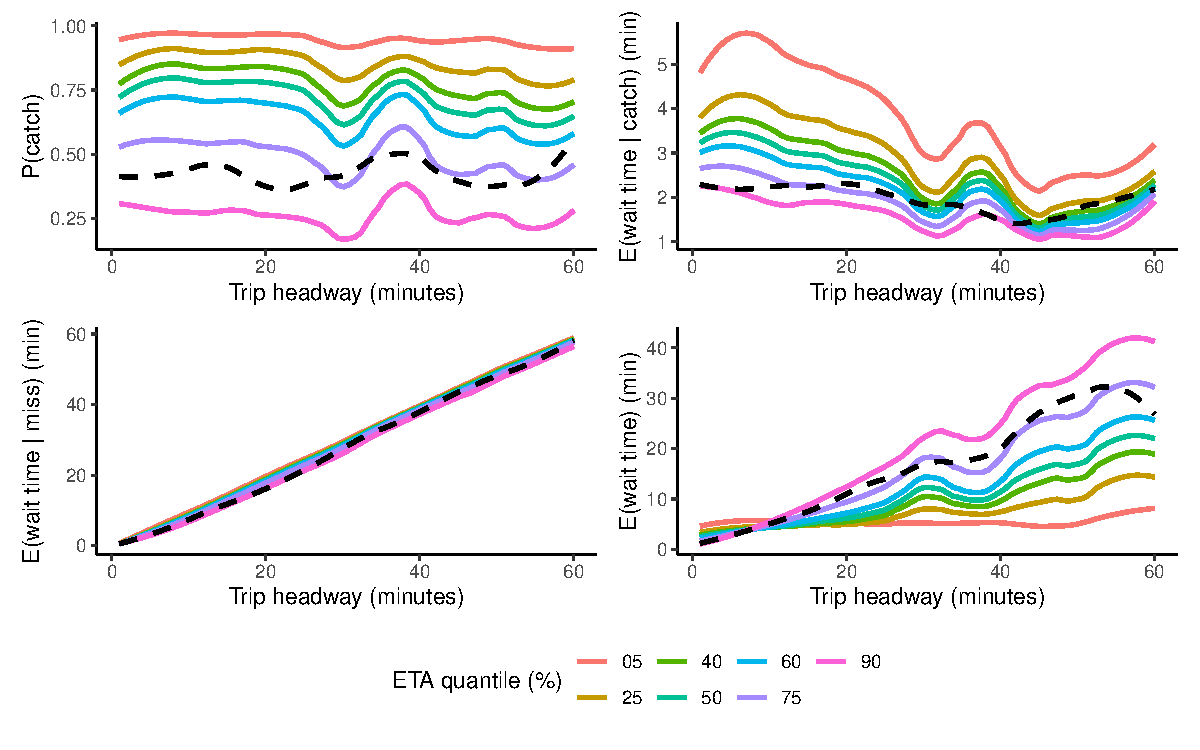
\includegraphics[width=\textwidth]{figure/eta_headway_results-1} 

}

\caption[Capture probabilities and expected wait times by trip headway]{Capture probabilities and expected wait times by trip headway (time until the next trip) using varying quantiles as point estimates of arrival time. Wait times assume the passenger arrives at the specified time. The dashed black line represents the same values using the schedule-delay prediction.}\label{fig:eta_headway_results}
\end{figure}


\end{knitrout}
